\textbf{קלט:}
גרף 
$G = (V, E)$
(מכוון או לא) וצומת מקור $s$.
\\
\textbf{מטרה:}
למצוא עץ עם שורש $s$,
$T = (U, F)$, 
$U \subseteq V$, 
$F \subseteq E$
כך ש-$U$ היא קבוצת הצמתים שישיגים מ-$s$.
בנוסף, לכל צומת
$u \in U$
נרצה ש-%
$p(u)$
יצביע לאבא של 
$u$.
\\
למשל:
\begin{center}
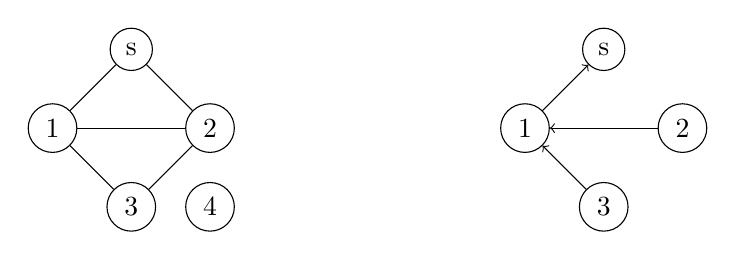
\begin{tikzpicture}[every node/.style={circle, draw, minimum width=5mm}]

\node(s) at(0,0) {s};
\foreach [count=\i] \x\y in {-1/-1,1/-1,0/-2,1/-2}{
	\node(\i) at(\x,\y) {\i};
}

\foreach \u \v in {
s/1%
,s/2%
,1/2%
,1/3%
,2/3%
}{
	\draw (\u) -- (\v);
}

\begin{scope}[xshift=6cm]
\node(s) at(0,0) {s};
\foreach [count=\i] \x\y in {-1/-1,1/-1,0/-2}{
	\node(\i) at(\x,\y) {\i};
}

\foreach \u \v in {
s/1%
,1/2%
,1/3%
}{
	\draw[<-] (\u) -- (\v);
}
\end{scope}

\end{tikzpicture}
\end{center}

\begin{definition}[חתך]
חתך בגרף,
$G = (V, E)$,
הוא תת קבוצה של צמתים. 
$S \subseteq V$
נאמר שקשת 
$uv \in E$
\emph{חוצה}
את החתך $S$ אם
$|\{u,v\} \cap S| = 1$.
\end{definition}

\begin{center}
\begin{tikzpicture}[every node/.style={default node}]
\foreach[count=\i] \x \y in {
	0/0
	,2/1
	,1/2
	,-1/1
	,-2/-1
}{
	\node(\i) at(\x, \y) {\i};
}

\foreach \u \v in {%
	5/4%
	,5/1%
	,4/1%
	,1/3%
	,4/3%
	,3/2%
}{
	\draw (\u) -- (\v);
}

\draw[blue, dashed, very thick]
(5.south) to[out=0, in=-135]
(4.south east) to[out=45, in=-90]
(3.east) to[out=90, in=45]
(4.north west) to[out=-135, in=180]
(5.south)
;
\end{tikzpicture}
\end{center}


\begin{enumerate}
\item 
אתחול:
$T \leftarrow \emptyset$, 
$U \leftarrow \{s\}$
ולכל 
$v \in V$
מציבים 
$p(v) \leftarrow \text{nil}$
\item
כל עוד יש קשת
$uv$
שחוצה את $U$ 
($u \in U$)
	\begin{enumerate}
	\item
	$U \leftarrow U \cup \{v\}$,
	$T \leftarrow T \cup \{uv\}$,
	$p(v) \leftarrow u$
	\end{enumerate}
\end{enumerate}

\begin{claim}
בסיום ריצת האלגוריתם
$U$
מכילה את כל הצמתים הישיגים מ-$s$
\end{claim}
\begin{proof}
בשלילה, בוחרים מסלול מ-$s$ לצומת $v$ שלא נכנס ל-%
$U$
ומסתכלים על הצומת הראשון במסלול שלא נכנס.
\end{proof}
\begin{claim}
בכל שלב בריצת האלגוריתם
$T$
עץ קשיר.
בנוסף המסלול מצומת $u$ ל-$s$ הוא שרשור של הקשת 
$(u, p(u))$
והמסלול מ-%
$p(u)$
ל-%
$s$
\end{claim}
\begin{proof}
באינדוקציה על צעד האלגוריתם.
\end{proof}
\begin{theorem}
בסיום ריצת האלגוריתם הכללי $T$ הוא עץ שפורש את כל הצמתים הישיגים מ-$s$
\end{theorem}







